
\subsection{Introduction}

Since Rubin's seminal work on multiple imputation (MI) \citep{rubin1978,rubin1979,rubin1987},
the method has been broadly applied, methodologically extended, and expanded towards ever more areas of application  \citep{carpenter2008,buuren12,carpenter2012,wim2015}.  {\color{black}{Multiple imputation is a commonly used approach to analyze incomplete data. A growing literature and increasing number of software implementations have contributed to the spread of the method. One of the attractions of MI is its very good to excellent performance even with a relatively small number of imputed datasets. This was important when Rubin created the method, about forty years ago, in view of, among others, the US Census. It still is today because of ever increasing data streams.}} 

Broadly, MI replaces a missing value with several plausible values, sampled from an appropriate predictive distribution for the missing values, given observed information. The method produces several completed datasets to replace the initial partially observed dataset.

An evident practical question is how many {\color{black}{imputed datasets}}, $M$ say, are sufficient for reliable results, knowing that full efficiency would be reached for $M=+\infty$. Precision should be balanced against computational expense. It has been stated repeatedly, and practically confirmed, that a small number of imputations oftentimes gives very acceptable results. Sources like \cite{rubin1987} and the classic \cite{littlerubin2002} quote values as low as 2--5. While attractive, especially when faced with large and complex databases, such low numbers may not always apply. Features that would require larger numbers of imputation include: increasing amounts of missing information, and the need for hypothesis testing rather than merely parameter and precision estimation. It is reassuring that \cite{schafer1997} indicated that, even under undesirable circumstances, it is rare for $M$ needing to be in excess of twenty. This observation was based on extensive simulation, rather than theory. 

Some of the approaches for dealing with selecting the number of imputations are reviewed in Section~\ref{sec_review}. Our proposal to handle the choice is presented in 
Section~\ref{sec_proposal}. Section~\ref{sec_simulations} reports some simulations, while real-life applications are offered in Section~\ref{sec_case_studies}. 



\subsection{Number of imputed datasets: A review}
\label{sec_review}
Upon producing multiply imputed datasets, a standard analysis is routinely applied to each of the completed datasets. Let $\bftheta$ be the parameter vector of interest and  $\widehat{\bftheta}_m$  its estimate from the $m$th imputed dataset. If $M$ is the number of {\color{black}{imputed datasets}}, then $\tilde{\bftheta}$, the multiple imputation estimator is defined as:
\begin{equation}
\label{est}
\widetilde{\bftheta}=\frac{1}{M} \sum_{m=1}^M \widehat{\bftheta}_m.
\end{equation}
If $\widehat{\Sigma}_m$ is the estimated variance-covariance of $\widehat{\bftheta}_m$, then the within-imputation variability is:
\begin{equation}
\label{M}
\widehat{W}=\frac{1}{M}\sum_{m=1}^M \widehat{\Sigma}_m,
\end{equation}
and the between-imputation variability is: 
\begin{equation}
\label{B}
\widehat{B} = \frac{1}{M-1}\sum_{m=1}^M \left (\widehat{\bftheta}_m - \widetilde{\bftheta} \right)\left (\widehat{\bftheta}_m - \widetilde{\bftheta} \right)'.
\end{equation}
Then, asymptotically, for the sample size as well as $M$ going to infinity, we have 
\begin{equation}
\label{large_M}
\widetilde{\bftheta}\sim N(\bftheta,\widehat{B}+\widehat{W}).
\end{equation} 
For finite $M$, the variance of the normal distribution in (\ref{large_M}) becomes \citep{littlerubin2002}:
\begin{equation}
\label{finite_M}
\widehat{V}=(1+M^{-1}) \widehat{B} + \widehat{W}.
\end{equation}
The term $\widehat{B}/M$ takes into account the increased variability stemming from finite $M$. Obviously, for $M\rightarrow \infty$, this extra term vanishes. Consider
{\color{black}{$r=\frac{1}{q}\left(\mathrm{tr}(\widehat{B}\widehat{W}^{-1})\right)(1+M^{-1})$ and $\nu = (M-1)(1+r^{-1})^2$ with $\mathrm{tr}(A)$ indicating the trace of the matrix $A$, and $q$ the length of parameter vector $\bftheta$}}. For the $k$th element of $\bftheta$ we have:
\begin{equation}
\label{theta_approx}
\widetilde{\theta_k} \approx \theta_k+ t_{\nu} \sqrt{\widehat{V_{kk}}},
\end{equation}
where $t_{\nu}$ is Student's $t$ distribution with $\nu$ degrees-of-freedom and $\widehat{V}$ can be computed using (\ref{finite_M}). These expressions are derived and discussed in detail by  \cite{rubin1987} or \cite{carpenter2012}. The degrees-of-freedom $\nu$ are computed by \cite{rubin1986_df}. Small sample degrees-of-freedom are reviewed by \cite{wagstaff2011}. Note that (\ref{theta_approx}) applies to the scalar case.

Now, if $I_M$ is the information based on $M$ imputations and $I_{\infty}$ is the information for $M\rightarrow+\infty$, then,
\begin{equation}
\label{relative_information}
\frac{I_M}{I_{\infty}} = \left( 1+ \frac{\gamma}{M} \right) ^{-1},\; \gamma=\frac{r+2/(\nu+3)}{r+1},
\end{equation}
where $\gamma$ in (\ref{relative_information}) can be regarded as the fraction of missing information. \cite{rubin1987} suggested that for many applications with a moderate amount of missingness, 3--5 imputations might well be sufficient. For example, using these expressions, with $10\%$ missingness, $M=3$ would provide about $97\%$ efficiency when compared with an infinite number of {\color{black}{imputed datasets}}. It is not surprising that this rule of thumb is relatively broadly accepted in practice. For example, according to SAS/STAT(R) 9.4 User's Guide, the default number of imputations in the MI procedure is set equal to 5.

 {\color{blue}{However, in the latest version of SAS (SAS/STAT(R) 14.1)  the default number of imputed datasets ({\tt{NIMPUTE}}) is increased to 25. Furthermore, following \cite{white2011}, an option is provided in this version of SAS' {\tt{PROC MI}} to set the number of imputed datasets equal to the fraction of incomplete cases ({\tt{NIMPUTE=PCTMISSING}}). This indicates a level of acceptance among commercial software developers for the need for larger $M$'s, also alternative procedures to determine it.}}

A practical difficulty with this heuristic is the need for $\gamma$. 
The quantity should be estimated to begin with, but obviously, the quality of this estimate is hugely affected by the number of {\color{black}{imputed datasets}} itself. Furthermore, as \cite{bodner2008} also suggests, the rule for the number of {\color{black}{imputed datasets}} would take into account three parameters:  $\widetilde{\bftheta}$, its variance, and the degrees-of-freedom of the Student's $t$ distribution. When one is interested in controlling the $p$-values when conducting hypothesis tests, or other quantities, then perhaps more imputations are needed \citep{harel2003,carpenter2008}.

\cite{carpenter2012} distinguished between two cases. Their proposal is to use a small number of {\color{black}{imputed datasets}} when the inference is clear-cut, but if it is less clear-cut and an accurate estimate of the $p$-value or $\gamma$ is needed, they proposed to set $M=100$.

Given that for small $M$, the approximation in (\ref{theta_approx}) may not be accurate enough, \cite{royston2004} proposed an iterative procedure to select $M$ such that the confidence level remains at a selected level. He proposed to select $M$ such that the coefficient of variation of $t_{\nu}\sqrt{\widehat{V_{kk}}}$ for the worst-case parameter becomes less than the type I error rate $\alpha$; this author used the conventional $\alpha=0.05$.

%\cite{hershberger2003} have derived a rather surprising result, motivated by structural equations problems. They treated the number of imputations as following a standard uniform distribution.  They brought into the equation a measure of required precision, much like in survey sampling theory: they placed a cap on the difference between the ``true" and predicted number of imputations. In their logic, with a confidence level of 95\% and an error between true and predicted number of imputations at most 10\%, they found that 510 imputations are needed. We consider their method less practically relevant because important aspects, such as the amount of missing information, target of inference, etc., are not taken into account. \cite{von2005} has refuted the proposal of \cite{hershberger2003} as well, but we mention it here as an example of different ways of looking at the problem of determining the number of imputations.

\cite{graham2007} have performed a simulation study to investigate the effect of $M$ on various characteristics, such as power, mean squared error, fraction of missingness, etc. \cite{bodner2008} explored various factors that are affected by increasing $M$. His findings were used in \cite{lu2014} who considered the case of longitudinal data and then focused on determining $M$ to stabilize MI-based inferences. Stability in these articles is defined in terms of four conditions regarding the conditional standard errors of the MI estimator, the test statistics, the missingness fraction, as well as the coefficient of variation of the half confidence interval. {\color{blue}{Under some circumstances, these authors proposed to use as many as $200$ imputed datasets.}}

{\color{black}{\cite{royston2009} proposed a jackknife procedure \citep{efron1981} to estimate $\sqrt{B/M}$, the so-called Monte Carlo error. These authors then propose to select the sufficient number of imputed datasets based on achieving a pre-defined level of precision. Their approach is implemented in the command {\ttfamily{mim}} in \textsc{Stata}.}} 

\subsection{Number of {\color{black}{imputed datasets}}: an alternative proposal}
\label{sec_proposal}
As we have seen, in most of the proposed rules for choosing $M$, the comparison is always between characteristics under a given, finite $M$ on the one hand, and $M\rightarrow+\infty$ on the other. In contrast, our proposal is to compare the quantity of interest with its successor (i.e., under $M$ versus $M+1$). As the estimated parameter and its variance using MI will converge to some asymptotic values as $M\rightarrow\infty$, monitoring this convergence is insightful. This implies an iterative perspective, which is convenient for practice. {\color{black}{We call this procedure the iterative multiple imputation (imi).}} The {\color{black}{imi}} procedure is formulated as follows:
\begin{enumerate}
{\color{black}{\item \textbf{Start.} Select an initial number of imputed datasets, $M_0$, {\color{blue}{$\widetilde{\bftheta}_{M_0} = \sum_{i=1}^{M_0} \widehat{\bftheta}_i/ M0.$}}
\item \textbf{Update.} For $m>M_0$,}} \begin{equation}
\label{update}
\widetilde{{\bftheta}}_{m+1}=\frac{m\widetilde{\bftheta}_m + \widehat{\bftheta}_{m+1}}{m+1}.
\end{equation}
\item \textbf{Distance.} Compute: $d_{m+1}=d(\widetilde{\bftheta}_{m+1},\widetilde{\bftheta}_{m})$ using an appropriate distance.
\item \textbf{Stopping rule.} {\color{black}{$d_{j} < \varepsilon$ for $j=m+1,\ldots,m+k_0$.}}
\end{enumerate}
{\color{black}{Here, $M_0$ is an integer indicating the initial number of imputations. For $M_0=2$, the stopping rule will be examined from the beginning, but in situations where the user knows a minimum number of imputations are needed (based on proportion of missing data, etc.) a larger $M_0$ can be used.}}  $\widehat{\bftheta}_m$ is the estimated parameter in the $m$-th iteration and $\widetilde{\bftheta}_m=\sum_{i=1}^ M \widehat{\bftheta}_m / M$. Note that $\widetilde{\bftheta}$ can be replaced with other quantities of interest, e.g., $p$-values. Clearly, for various quantities of interest, the corresponding combination rule should be applied in (\ref{update}). {\color{black}{Since the convergence of this procedure is not monotone, one needs to determine an integer $k_0$ as the number of successive steps that the stopping rule should be validated. This would prevent an early declaration of convergence. Again, $k_0=1$ would stop the first time this criterion is met, but a larger $k_0$ is recommended. Our proposal is to use $k_0=3$ (see Sections \ref{sec_simulations} and \ref{sec_conclusions}).

As can be seen, the number of imputed datasets in the proposed iterative procedure has two components: a deterministic part: $M_0+k_0$ and a stochastic part which is determined by the iterations. Our implementation of this procedure in \textsc{R} package {\ttfamily{imi}} makes it possible to determine these two parameters interactively after observing the computation time of imputing the dataset and fit the model for $M0=2$ times.}} 


{\color{black}{According to the convergence rate of the multivariate central limit theorem \citep{gotze1991,berckmoes2016}, roughly speaking, the convergence of $\widetilde{\bftheta}$ to $\theta$ as $M\rightarrow\infty$ in (\ref{large_M}) depends on 3 different aspects: sample size, dimension of the random vector (parameter space), and the third moment of the components of the random vector. In our iterative procedure, the sample size consists of two aspects: the number of imputed datasets, $M$, also the proportion of missing data. A larger $M$ makes the convergence faster, while a larger proportion of missing data makes it slower. On the other hand, another important issue is the dimension of the parameter space, the more parameters to estimate the more slowly the convergence will be achieved. The third moment highlights the role of the model, for example, the convergence for a linear model would be different from a logistic regression (see Section~\ref{sec_simulations}). Therefore, an appropriate method for determining $M$ should consider all these aspects. In other words, it should be sensitive to changes in any of these factors. As our proposed method uses the goal of the analyses (parameter estimate, hypothesis testing, etc.) in the process of determining $M$, it includes such aspects. Simulation results in Section~\ref{sec_simulations} support this claim as well.}}

One important aspect of the proposed iterative procedure is the choice of an appropriate distance in Step 3. One immediate choice is to use an Euclidean distance, as follows:
\begin{equation}
\label{relative_euc}
d_{m+1}^{\mathrm{Euc}}=\sqrt{\left(\widetilde{\bftheta}_{m+1}- \widetilde{\bftheta}_{m}\right)^T\left(\widetilde{\bftheta}_{m+1}- \widetilde{\bftheta}_{m}\right)}.
\end{equation}
%$d_{m+1}^{\mathrm{Euc}}$ depends on the length of the vector of interest. Therefore, one may use $d_{m+1}^{\mathrm{Euc}}/k$ instead, where $k$ is the length of vector $\bftheta$. 
Alternatively, one may try to make the largest difference smaller, then an $\ell_{\infty}$-norm would be the appropriate distance. 
%While $d_{m+1}^{\mathrm{Euc}}/k$ is a compromise distance measure, $\ell_{\infty}$-norm is more stringent. 
Obviously, for {\color{black}{$q=1$}} these two are equivalent:
\begin{equation}
\label{infinity_norm}
d_{m+1}^{\ell_{\infty}}= \max\left\{ |\widetilde{\bftheta}_{m+1}- \widetilde{\bftheta}_{m}|\right\}.
\end{equation}
The common problem with $\ell_p$-norm type distance measures in (\ref{relative_euc})--(\ref{infinity_norm}) is the fact that they would emphasize the elements in the parameter vector which have larger magnitude. Also, they are not robust against changes in units. {\color{black}{This can also be seen from the general definition of the $\ell_p$-norm of a vector $\mathbf{x} = (x_1,\ldots,x_k)$, $\|\mathbf{x}\|_p$:
\begin{equation*}
\|\mathbf{x}\|_p = \left(|x_1|^p + \ldots+ |x_k|^p\right) ^{1/p}, p\leq 1.
\end{equation*}
When $p\rightarrow\infty$, one can show:
\begin{equation*}
\|\mathbf{x}\|_{\infty}=\max\{|x_1|,\ldots,|x_k| \}.
\end{equation*}}}
As an alternative, we propose using the Mahalanobis distance \citep{mahalanobis1936}: 
\begin{equation}
\label{mal_dis}
d_{m+1}^{\mathrm{Mah}} = \sqrt{\left(\widetilde{\bftheta}_{m+1}- \widetilde{\bftheta}_{m}\right)^T S^{-1} \left(\widetilde{\bftheta}_{m+1}- \widetilde{\bftheta}_{m}\right)}.
\end{equation}
{\color{black}{For using (\ref{mal_dis}), one needs to define an appropriate $S$. One can show:
\begin{equation}
\label{diff_cov}
\widetilde{{\bftheta}}_{m+1}-\widetilde{{\bftheta}}_m = \frac{\widehat{\bftheta}_{m+1}- \widetilde{{\bftheta}}_m}{m+1}.
\end{equation}
Considering the fact that $\widehat{\bftheta}_{m+1}$ and $\widetilde{{\bftheta}}_m$ are independent given the observed part of the sample, one may use:
\begin{equation}
\label{diff_cov}
\mathrm{Cov}\left(\frac{\widehat{\bftheta}_{m+1}- \widetilde{\bftheta}_m}{m+1} \right)=\frac{1}{(m+1)^2}\left[\mathrm{Var}(\widehat{\bftheta}_{m+1})+[\mathrm{Var}(\widetilde{\bftheta}_{m})\right] = \frac{1}{(m+1)^2}[\mathrm{Var}(\widehat{\theta}_{m+1})+\widehat{W}_m].
\end{equation}
The division by $m+1$ in (\ref{diff_cov}) makes this an inappropriate candidate for $S$, as it changes every time, while we need to monitor convergence of the procedure, relative to a sufficiently stable yardstick. 

Other choices for $S$ include the within, between, or combined covariance matrix of the parameters at step $m+1$, i.e., $\widehat{W}_{m+1}$, $\widehat{B}_{m+1}$, or $\widehat{V}_{m+1}$, respectively; here $\widehat{V}$ is computed as in \ref{finite_M}.}}
%Considering the fact that $\widetilde{\bftheta}_{m+1}$ and $\widetilde{\bftheta}_{m}$ are independent given the observed part of the sample, one may use,
%\begin{equation}
%\label{mal_all}
%S=\widehat{V}_{m+1}+\widehat{V}_{m},
%\end{equation}
%where $\widehat{V}$ is computed as in \ref{finite_M}. Another choice for $S$ would only use the between variability of $\widehat{\theta}_m$'s $(m=1,\ldots,M)$,
%\begin{equation}
%\label{mal_between}
%S=\widehat{B}_{m+1} + \widehat{B}_{m}.
%\end{equation}
{\color{black}{Our simulation results show that $\widehat{B}_{m+1}$ cannot be an appropriate choice since being normalized by the variability of the differences, the resulting Mahalanobis distance is not sensitive to the fraction of missing data. This will be discussed in more detail in Section \ref{sec_simulations}.}} 

{\color{black}{An appropriate distance should be sensitive to the fraction of missing data, but robust against rescaling model parameters. Both $\widehat{W}$ and $\widehat{V}$ serve these purposes, but our simulation results show that (see Section~\ref{sec_simulations}) for some large values of variance components, $\widehat{W}$ would show chaotic behavior from one iteration to another in some cases, while $\widehat{V}$ balances between and within variability, hence behave more stably. Therefore, our proposal for an appropriate distance in Step 3 is the Mahalanobis distance with $S=\widehat{V}_{m+1}$.}} In cases where the quantity of interest is unitless, e.g., a correlation coefficient, a coefficient of variation, a coefficient of determination, a $p$-value, etc., using $\ell_p$-norm type distances such as in (\ref{relative_euc})--(\ref{infinity_norm}) is recommended, especially when obtaining the variance of the quantity of interest is not straightforward. Of course, one may use any tailored distance according to the problem at hand, {\color{black}{this}} would not change the proposed iterative procedure.

{\color{black}{As mentioned earlier, the convergence speed of the imi procedure depends on various factors such as the model, the parameter space, and the fraction of missing data. Also, the choice of the distance in Step 3 of the procedure plays a determining role when it comes to deciding when to stop. Therefore, formulating a fixed universal threshold for $\epsilon$ in Step 3 of the proposed iterative procedure seems not to be possible. However, based on extensive simulation results, when using a Mahalanobis-types distance as in (\ref{mal_dis}) with $S=\widehat{V}_{m+1}$, considering $\epsilon=0.05$ leads to a liberal choice of $M$. If one wants to select a conservative $M$, we propose to set $\epsilon=0.01$. In the same setting, such choices of $\epsilon$ would select $M$'s that are approximately in agreement with Rubin's classic suggestion, e.g., to use $M=5$ for $10\%$ missing data (See Table~\ref{tab_mvn}).}}

{\color{black}{In general, for selecting $\epsilon$}}, one needs to consider the nature of the quantity of interest when deciding on $\epsilon$. For example, when dealing with $p$-values, one needs to ensure that increasing the {\color{black}{number of imputed datasets}} would not change the result of the test, so the distance between two $p$-values from imputed datasets number $m$ and $m+1$, near or smaller than the significance, $\alpha$, should be smaller than, for example, $\alpha/10$; see Section~\ref{sec_les}.     {\color{black}{Therefore, in case of $p$-values, we propose to use a Euclidean distance with $\epsilon=\alpha/10$. Note that, given the null hypothesis, the $p$-value is uniformly distributed. Therefore, for an appropriate $\epsilon$ and up to a constant coefficient, using a Mahalanobis distance is equivalent to the Euclidean distance.}}

 {\color{blue}{As \cite{wald1939} pointed out, the two central procedures in theory of statistics are parameter estimation and hypothesis testing. To summarize our discussion above, we proposed to use a different $\epsilon$ for each of these procedures. In case of parameter estimation one may use $0.05$ or $0.01$, and in case of hypothesis testing (using $p$-values) one may use $\alpha/10$.}}


%When the fraction of missingness is large, it is possible that the convergence plot becomes too noisy. In such cases one may use an appropriately smoothed curve to decide on the number of imputations. To avoid the possible dangers of overcorrection, one may consider different smoothing methods and compare their results as a sensitivity analysis. In case different smoothing methods lead to almost the same conclusion, a final decision on $M$=1 can be made; see Section~\ref{sec_armd}.


\subsection{Simulation study}
\label{sec_simulations}

{\color{black}{In order to study our proposed method, two simulation plans are considered. One with a multivariate normal vector, and the other with a logistic regression model. Using these two simulation settings, the performance of our proposed procedure for both parameter estimation and hypothesis testing will be studied. The results will be displayed, compared, and discussed, after presenting the plans.}}

{\color{black}{
\subsubsection{Simulation plan}

A simulation study is undertaken for a multivariate normal vector as well as data generated from a logistic regression model. Two types of covariance structures are considered for the multivariate normal model: compound-symmetry (CS) and first--order autoregressive (AR(1)). Consider $\BY_i$ a vector of length $k$, then $\BY_i\sim N(\mu \mathbf{1}_{k}, \Sigma)$. Under CS, $\Sigma=\sigma^2I_{k}+\tau J_{k}$, for $\sigma^2,\tau >0$ and $I_{k}$ and $J_{k}$ the identity and all-ones matrices, respectively. For AR(1), we have $\Sigma=\sigma^2 C$ where the $(i,j)$ element of $C$ is defined as $\rho^{|i-j|}$, for $\sigma^2>0,-1\leq \rho \leq +1$. 

All data are generated for $\mu=0$. The length of each random vector is set to 5, and the sample size is considered to be 100. For each covariance structure in the multivariate normal case 18 different scenarios are considered as combinations of the following settings:

\begin{itemize}
	\item Two proportions of missing data are used: $10\%$ and $70\%$;
	\item Three $\sigma^2$ values are used: $1,16,64$;
	\item Three $\rho$ values are used: $0.2, 0.5, 0.8$. In case of CS, the corresponding $\tau$ is computed given the specified $\rho$ using $\tau=\rho\sigma^2/(1-\rho)$.
\end{itemize}
Logistic regression data are generated with parameters $(\beta_0,\beta_1,\beta_2)=(0.2,-2,0.5)$, where the design matrix is generated using each of the 9 considered CS settings. The parameters of the CS and AR(1) models are estimated using the results in \cite{hermans2017_cs} and \cite{hermans2017_ar1}, respectively. The logistic regression is fitted using \textsc{R} function {\tt{glm}}. The proportion of missing values are the same as in the multivariate normal scenarios ($10\%$ and $70\%$). 

The missing data for all of these scenarios are generated under a missing at random (MAR) mechanism using the function {\ttfamily{ampute}} in the \textsc{R} package {\ttfamily{mice}}{\color{blue}; see {\cite{ampute} and \cite{schouten2018}. The function {\tt{ampute}} implements a multivariate approach to generate missing data by assigning a weight to each observation. In case of a missing at random (MAR) mechanism, these weights only depend on the observed part of the sample. Based on the assigned weights, a logistic distribution will be used to compute the probability of missingness. An observation with a larger weight has more chance to be missing.}}




Each incomplete dataset is imputed $500$ times using a multivariate normal predictive model in the \textsc{R} package {\tt{Amelia2}}, and each scenario is repeated 100 times as well.

%Let us briefly describe how the function {\ttfamily{ampute}} works. It starts by considering different schemes of missingness. A scheme of missingness is a vector of $1$'s and $0$'s. The length of this vector is the same as the number of variables in the dataset. For a specific subject, $1$ means that the corresponding variable is recorded, and $0$ means it is possibly missing. Corresponding to each scheme of missingness, a set of weights will be considered that specifies the importance of each variable in determining whether a subject should contain missing values or not. Under an MAR mechanism, the variable with a missing value ($0$ in the scheme matrix) should have weight $0$, since it should not play a role in determining whether a missing should happen or not, this will be determined by observed variables. For each subject, based on the observed values and allocated weights, a weighted sum of scores is computed. These scores are used in a logit function to determine the probability of being missing or not. Obviously, this would lead to occurrence of various missing data patterns. More details can be found in \cite{ampute}.
%



To compute the distance between two steps in our iterative procedure, we use five different measures: Euclidean distance (\ref{relative_euc}), $\ell_{\infty}$-norm (\ref{infinity_norm}), Mahalanobis distance (\ref{mal_dis}) with $S$ selected as within ($\widehat{W}$), between ($\widehat{B}$), and combined covariance matrix ($\widehat{V}$) of the estimated parameter vector. 


There are two main outcomes of interest from different considered scenarios. First, the convergence plot for different distances. Second, the $M$ for which the iterative procedure terminates. Such $M$ is computed using seven values $\epsilon= 0.005, 0.01, 0.02, 0.03, 0.04$ and $0.05$, and for each $\epsilon$, three successive validation steps are considered: $k_0=1,3$ and $5$. 


In order to evaluate our proposed method in case of $p$-values, one-sample $t$-tests are applied with $H_0:\mu=d_0$ on the first column of the data generated from each setting of CS and AR(1) covariance structure. In addition, paired $t$-tests are also performed for testing $H_0:\mu_1-\mu_2=d_0$ for the first and the second columns of data generated using each setting of CS and AR(1) covariance matrices. To see the effect of the test value on the convergence, we have considered $d_0=0$ and $d_0=10$. As the $p$-value is a scalar, we use Euclidean distance (\ref{relative_euc}) to measure distance of two successive steps. In case of $p$-values, again the convergence plots are provided; also, the sufficient number of imputed datasets is computed for two values of $\epsilon=0.05/10$ and $0.05/100$. For each $\epsilon$, three successive validation steps are considered: $k_0=1,3$ and $5$. 

\subsubsection{Simulation results}
As displaying the results of 18 different scenarios takes a lot of space, here we discuss all of the outcomes but only display the results for one of them. The rest of the results will be available in the \textsc{R} package {\tt{imi}} via 9 lists of datasets, the function {\tt{imi.make.plots}} can be used to produce similar plots as in Figure~\ref{fig_mvn} and Figure~\ref{fig_ttest} for other scenarios. Further information can be found in the documentation of the package.

Figure~\ref{fig_mvn} shows the convergence plots for the scenario with $\sigma^2=16$ and $\rho=0.5$. As one may see, while using all of the distance functions a decreasing trend can be observed, but as expected Euclidean and $\ell_{\infty}$ norms, as well as Mahalanobis distance with $S=\widehat{B}$ are not performing well. On the other hand, the latter with both $S=\widehat{W}$ and $S=\widehat{V}$ performs fine. {\color{blue}{Note that for $70\%$ missing data for some of the imputed datasets, quasi-complete separation occurs when fitting logistic regression. In such cases, a new imputed dataset is generated.}} 

An interesting observation from Figure~\ref{fig_mvn} is the different convergence rate for logistic regression compared with the multivariate normal case. As one may see, for $10\%$ missing data, the logistic regression converges almost with the same speed as $70\%$ missing data in case of a multivariate normal vector parameter estimates. That highlights the effect of the model (thus not only the proportion of missing data) when determining a sufficient number of imputed datasets.



\begin{figure*}
	\centering
	\includegraphics[width=\textwidth]{figMMest.eps}
	\caption{Convergence plots for multivariate normal random vectors parameter estimates with CS and AR(1) covariance matrix structures (with $\sigma^2=16$ and $\rho=0.5$), as well as a logistic regression model, using five different distance functions: Euclidean norm, $\ell_{\infty}$-norm, and Mahalanobis distance with within, between, and combined covariance matrices over imputed sets of data for two proportion of missing data: $10\%$ and $70\%$. Each point in the plot is the average over 100 replications. {\color{blue}{The three horizontal dashed lines are $\epsilon = 0.05, 0.01, 0.001$, respectively.}}}
	\label{fig_mvn}
\end{figure*} 


Figure~\ref{fig_ttest} shows the convergence plots using $M=500$ for the $p$-values of one sample and paired $t$-tests for two different test values (0, 10). The distance between two $p$-values is computed using the Euclidean distance. As one may see, one important factor that should be taken into account when determining $M$ is the test value. When it is far from the actual parameter convergence is achieved for a much smaller $M$. 

\begin{figure*}
	\centering
	\includegraphics[width=\textwidth]{figttestMM.eps}
	\caption{Convergence plots for the $p$-values of one sample (first row) and paired (second row) $t$-tests for different values of test statistics. The data are generated from a (multivariate) normal distribution with mean $0$ and CS and AR(1) covariance matrices (with $\sigma^2=16$ and $\rho=0.5$). The missing values are generated with proportions $10\%$ and $70\%$. {\color{blue}{The two horizontal dashed lines are $\epsilon = 0.005, 0.0005$, respectively.}}}
	\label{fig_ttest}
\end{figure*} 


To explore the selected $M$ using various $\epsilon$'s and $k_0$'s to evaluate our proposals ($\epsilon=0.01$ or $0.05$, and $k_0=3$), Tables~\ref{tab_mvn} and \ref{tab_ttest} show the selected $M$ for parameter estimation in multivariate normal and logistic regression (Table~\ref{tab_mvn}) and $p$-values of one sample and paired $t$-tests (Table~\ref{tab_ttest}). As one may see, again the effect of proportion of missing data and the model is verified on the selected sufficient $M$. {\color{blue}{While a dataset with a larger proportion of missing data needs a larger $M$, the number of sufficient imputed datasets in case of logistic regression is different from multivariate normal, even for a smaller proportion of missing data. This would highlight the role of a procedure that accounts for all of these aspects.}}


Also, it seems that our proposals for $\epsilon$ and $k_0$ are sensible in terms of comparing with Rubin's classical rule suggesting 3--5 imputed datasets for $10\%$ missing data. In case of $p$-values it seems $\epsilon=0.005$ together with $k_0=3$ works acceptably fine.


{\color{blue}{An interesting observation when comparing the selected $M$ for different values of $\rho$ is the effect of \emph{missing information}. For the same fraction of missing data, when the correlation is larger, the selected $M$ is smaller. That would suggest that what really matters is not only the fraction of missing data, but the fraction of missing information.  As an extreme case, consider two variables $X$ and $Y$ in a given dataset, suppose $X$ is complete and $Y$ is partially missing. Assume further that $Y_i = X_i$ ($\rho = 1$), for every subject. In this case one imputation would be sufficient, no matter the fraction of missing items. Figure~\ref{fig_missinfo} shows the selected $M$ for different scenarios with $\sigma^2 = 16$ and $\rho = 0.5$ and $0.8$, and $k_0 = 3$
. As one may see, in most of the cases, for the same proportion of missing data and model, the selected $M$ is smaller when $\rho$ is larger.}}



\begin{table}[ht]
	\caption{Mean, standard deviation (STD) for selected $M$ given different $\epsilon$ and $k_0$ values, and number of times $M>500$ (out of 100 replications) for different models and different $\epsilon$'s using the Mahalanobis-type distance with $S=\widehat{V}$. The results are presented for 3 different successive validation steps $k_0=1, 3, 5$.}
	\label{tab_mvn}
	\centering
\resizebox{\textwidth}{!}{	\begin{tabular}{lcccccccccc}
		\hline
\multirow{2}{*}{Model}	&	\multirow{2}{*}{$\epsilon$} & \multicolumn{3}{c}{$k_0=1$} &  \multicolumn{3}{c}{$k_0=3$} &  \multicolumn{3}{c}{$k_0=5$} \\ 
	&	& Mean & STD & $M>500$ & Mean & STD & $M>500$ & Mean & STD & $M>500$\\ 

  \hline
\multirow{6}{*}{CS-$10\%$}  &0.005 & 13.82 & 5.02 & 0.00 & 29.16 & 8.54 & 0.00 & 37.63 & 9.24 & 0.00 \\ 
  &0.01 & 7.15 & 3.08 & 0.00 & 15.38 & 4.88 & 0.00 & 19.31 & 6.01 & 0.00 \\ 
  &0.02 & 3.88 & 1.96 & 0.00 & 6.98 & 3.05 & 0.00 & 8.62 & 3.64 & 0.00 \\ 
  &0.03 & 2.67 & 1.44 & 0.00 & 4.36 & 2.22 & 0.00 & 5.31 & 2.51 & 0.00 \\ 
  &0.04 & 2.09 & 1.06 & 0.00 & 3.27 & 1.71 & 0.00 & 3.63 & 1.91 & 0.00 \\ 
  &0.05 & 1.68 & 0.84 & 0.00 & 2.42 & 1.51 & 0.00 & 2.78 & 1.80 & 0.00 \\ \hline
\multirow{6}{*}{CS-$70\%$}   &0.005 & 30.71 & 10.28 & 0.00 & 71.12 & 13.25 & 0.00 & 94.98 & 14.39 & 0.00 \\ 
  &0.01 & 18.12 & 5.24 & 0.00 & 37.93 & 8.01 & 0.00 & 50.62 & 9.72 & 0.00 \\ 
  &0.02 & 10.06 & 3.74 & 0.00 & 20.73 & 5.33 & 0.00 & 25.04 & 5.41 & 0.00 \\ 
  &0.03 & 6.45 & 2.59 & 0.00 & 13.65 & 3.95 & 0.00 & 16.85 & 4.39 & 0.00 \\ 
  &0.04 & 4.81 & 2.10 & 0.00 & 9.61 & 3.03 & 0.00 & 12.24 & 3.78 & 0.00 \\ 
  &0.05 & 3.94 & 1.94 & 0.00 & 7.67 & 2.70 & 0.00 & 9.40 & 3.18 & 0.00 \\ \hline
\multirow{6}{*}{AR(1)-$10\%$}  &0.005 & 18.86 & 7.24 & 0.00 & 39.05 & 11.13 & 0.00 & 46.60 & 12.93 & 0.00 \\ 
  &0.01 & 10.37 & 4.28 & 0.00 & 18.72 & 6.58 & 0.00 & 23.81 & 8.44 & 0.00 \\ 
  &0.02 & 4.99 & 2.33 & 0.00 & 9.85 & 3.57 & 0.00 & 11.74 & 4.29 & 0.00 \\ 
  &0.03 & 3.45 & 1.59 & 0.00 & 5.96 & 2.77 & 0.00 & 7.44 & 3.33 & 0.00 \\ 
  &0.04 & 2.40 & 1.22 & 0.00 & 4.15 & 2.29 & 0.00 & 4.67 & 2.54 & 0.00 \\ 
  &0.05 & 2.03 & 1.07 & 0.00 & 3.02 & 1.65 & 0.00 & 3.64 & 2.15 & 0.00 \\ \hline
\multirow{6}{*}{AR(1)-$70\%$}  &0.005 & 44.30 & 13.06 & 0.00 & 97.12 & 17.89 & 0.00 & 123.94 & 20.28 & 0.00 \\ 
  &0.01 & 23.71 & 8.08 & 0.00 & 51.85 & 9.49 & 0.00 & 64.14 & 11.04 & 0.00 \\ 
  &0.02 & 13.55 & 4.93 & 0.00 & 26.79 & 6.21 & 0.00 & 33.91 & 6.82 & 0.00 \\ 
  &0.03 & 9.28 & 3.36 & 0.00 & 17.81 & 3.97 & 0.00 & 21.94 & 5.11 & 0.00 \\ 
  &0.04 & 6.76 & 2.65 & 0.00 & 13.59 & 3.34 & 0.00 & 16.67 & 3.93 & 0.00 \\ 
  &0.05 & 5.44 & 2.26 & 0.00 & 10.84 & 2.98 & 0.00 & 13.12 & 3.17 & 0.00 \\ \hline
\multirow{6}{*}{Logreg-$10\%$}  &0.005 & 39.06 & 16.12 & 0.00 & 71.73 & 24.19 & 0.00 & 90.08 & 29.32 & 0.00 \\ 
  &0.01 & 19.95 & 8.71 & 0.00 & 38.31 & 14.02 & 0.00 & 46.67 & 15.70 & 0.00 \\ 
  &0.02 & 11.14 & 5.26 & 0.00 & 20.38 & 7.42 & 0.00 & 25.47 & 9.62 & 0.00 \\ 
  &0.03 & 7.31 & 3.60 & 0.00 & 13.06 & 5.50 & 0.00 & 16.28 & 6.07 & 0.00 \\ 
  &0.04 & 5.36 & 2.82 & 0.00 & 9.98 & 4.10 & 0.00 & 11.72 & 4.71 & 0.00 \\ 
  &0.05 & 4.60 & 2.56 & 0.00 & 7.85 & 3.38 & 0.00 & 9.53 & 3.78 & 0.00 \\ \hline
\multirow{6}{*}{Logreg-$70\%$}  &0.005 & 61.33 & 26.34 & 0.00 & 140.31 & 53.29 & 0.00 & 174.82 & 67.77 & 0.00 \\ 
  &0.01 & 36.68 & 15.25 & 0.00 & 76.05 & 25.85 & 0.00 & 94.65 & 32.48 & 0.00 \\ 
  &0.02 & 21.35 & 7.88 & 0.00 & 40.75 & 13.77 & 0.00 & 51.16 & 16.31 & 0.00 \\ 
  &0.03 & 14.68 & 6.37 & 0.00 & 28.97 & 8.96 & 0.00 & 34.92 & 10.65 & 0.00 \\ 
  &0.04 & 11.76 & 4.29 & 0.00 & 22.35 & 6.44 & 0.00 & 26.23 & 7.47 & 0.00 \\ 
  &0.05 & 10.01 & 4.00 & 0.00 & 18.99 & 5.44 & 0.00 & 21.77 & 6.26 & 0.00 \\ 
   \hline
\end{tabular}}
\end{table}


\begin{table}[ht]
	\caption{Mean, standard deviation (STD) for selected $M$ given different $\epsilon$ and $k_0$ values, and number of times $M>500$  for different models and different $\epsilon$'s for $t$-test and paired $t$-test with test value $\mu=0$. The results are presented for 3 different successive validation steps $k_0=1, 3, 5$.}
	\label{tab_ttest}
	\centering
\resizebox{\textwidth}{!}{	\begin{tabular}{clcccccccccc}
		\hline
\multirow{2}{*}{Test}&	\multirow{2}{*}{Model}&\multirow{2}{*}{$\epsilon$} & \multicolumn{3}{c}{$k_0=1$} &  \multicolumn{3}{c}{$k_0=3$} &  \multicolumn{3}{c}{$k_0=5$} \\ 
&&& Mean & STD & $M>500$ & Mean & STD & $M>500$ & Mean & STD & $M>500$ \\ 
		\hline
\multirow{8}{*}{$\mu1=0$} &\multirow{2}{*}{CS-$10\%$}  &0.005 & 2.90 & 2.55 & 0.00 & 8.17 & 6.74 & 0.00 & 11.32 & 8.93 & 0.00 \\ 
 & &5e-04 & 12.78 & 9.70 & 0.00 & 50.41 & 32.28 & 0.00 & 83.97 & 53.85 & 0.00 \\ 
&\multirow{2}{*}{CS-$70\%$}  &0.005 & 5.41 & 3.85 & 0.00 & 20.22 & 10.08 & 0.00 & 29.20 & 14.79 & 0.00 \\ 
 & &5e-04 & 21.75 & 12.38 & 0.00 & 119.70 & 57.55 & 0.00 & 211.70 & 93.22 & 0.00 \\ 
 &\multirow{2}{*}{AR(1)-$10\%$}  &0.005 & 2.76 & 2.03 & 0.00 & 7.55 & 6.39 & 0.00 & 10.55 & 9.08 & 0.00 \\ 
 & &5e-04 & 12.73 & 10.51 & 0.00 & 53.61 & 34.37 & 0.00 & 88.68 & 63.04 & 0.00 \\ 
  &\multirow{2}{*}{AR(1)-$70\%$} &0.005 & 5.91 & 4.34 & 0.00 & 20.98 & 10.62 & 0.00 & 30.73 & 15.85 & 0.00 \\ 
  &&5e-04 & 22.88 & 15.28 & 0.00 & 120.90 & 57.80 & 1.00 & 214.83 & 97.30 & 1.00 \\ \hline

\multirow{8}{*}{$\mu1-\mu_2=0$} &\multirow{2}{*}{CS-$10\%$}    &0.005 & 3.32 & 2.24 & 0.00 & 10.34 & 7.32 & 0.00 & 15.16 & 11.30 & 0.00 \\ 
  &&5e-04 & 15.75 & 11.31 & 0.00 & 64.97 & 37.27 & 0.00 & 110.12 & 58.83 & 0.00 \\ 
 &\multirow{2}{*}{CS-$70\%$}  &0.005 & 6.62 & 4.14 & 0.00 & 25.41 & 13.59 & 0.00 & 36.49 & 19.45 & 0.00 \\ 
  &&5e-04 & 25.94 & 17.69 & 0.00 & 157.88 & 74.58 & 6.00 & 243.37 & 124.17 & 6.00 \\ 
  &\multirow{2}{*}{AR(1)-$10\%$}  &0.005 & 4.02 & 2.78 & 0.00 & 11.46 & 7.58 & 0.00 & 16.18 & 10.01 & 0.00 \\ 
 & &5e-04 & 14.37 & 10.65 & 0.00 & 74.38 & 40.09 & 0.00 & 134.99 & 70.34 & 0.00 \\ 
   &\multirow{2}{*}{AR(1)-$70\%$}&0.005 & 8.31 & 5.11 & 0.00 & 29.14 & 14.83 & 0.00 & 43.30 & 19.48 & 0.00 \\ 
 & &5e-04 & 31.39 & 17.23 & 0.00 & 160.09 & 72.00 & 2.00 & 288.81 & 112.58 & 2.00 \\ 
	\end{tabular}}
\end{table}


}}


\begin{figure*}
	\centering
	\includegraphics[width=\textwidth]{figMisisngInformation.eps}
	\caption{Averaged selected $M$ with $k_0 = 3$ for data generated from a multivariate normal with mean 0 and covariance matrix with CS and AR(1) structures with  $\sigma^2 =16$ and $\rho = 0.5, 0.8$, as well as a logistic regression model. The proportions of missing data are $10\%$ and $70\%$. Each point in the plot is the average over 100 replications.}
	\label{fig_missinfo}
\end{figure*} 


{\color{black}{

\subsection{Applications}
\label{sec_case_studies}
In this section, two applications of multiple imputations are considered: fitting a logistic regression to incomplete data, as well as combining $p$-values from a one-sample $t$-test for a set of incomplete data. The number of imputed datasets will be determined using the proposed iterative procedure via the \textsc{R} package {\ttfamily{imi}}.


\subsubsection{Leuven Eye Study. Logistic regression}
\label{sec_les}
The Leuven Eye Study \citep[LES;][]{abegao2015}, is an extensive observational study of glaucoma performed at the ophthalmology department of UZ Leuven. The dataset so far consists of 141 variables measured for 585 subjects. As this study was performed in a clinical setting, it was not feasible to measure all these variables for all of the subjects. Because of that, missingness is a considerable problem. Among these 141 variables, 130 of them are selected to be used in multiple imputation. An analysis was performed to study which risk factors are relevant for the binary outcome defined as normal vs. glaucoma. The risk factors selected for the model include both structural and functional measurements of the eye (cup to disc ratio, corneal thickness, visual acuity), previous medical history (gender, sleep apnea, rhythm disorder, having had cataract surgery, being medicated with statins or calcium channel blockers) and more variable biometric measurements, like intra-ocular pressure and diastolic blood pressure.

Figure~\ref{fig_conv_real} (bottom-left) shows a histogram of the number of missing values (out of 585 patients) in the LES dataset. As one may see, the number of missing values is diverse. Also the patterns of missing values could be different from variable to variable. Therefore, determining $M$ using classical or simulation-based approaches could be a challenge here. Using our proposal, it could be more convenient to determine the sufficient number of imputed datasets.

Considering the size of the dataset as well as various variable types, in order to impute the missing values the fully conditional specification (FCS) approach \citep[and \citealp{van2006}]{van2007,buuren12} is employed. For continuous variables, predictive mean matching, \cite{little1988}, is used for generating the imputed datasets. Also, a binary logistic regression predictive model is used to impute binary variables. In the specific case of one variable with three levels, a polytomous logistic regression predictive model is used. 
In order to create a sufficient number of imputed datasets we use the function {\ttfamily{imi.glm}} in the \textsc{R} package {\ttfamily{imi}}.

%\noindent{\ttfamily{regressors=c("Sleepapnea", "C\_vs\_D","RithmDisor","DBP","VA\_log\_mar","IOP\_DCT","Phaco",
%		"Statinany",\\"CCBany","CCT","SEX") \\
%		resp='Diagnosis5.bin'\\
%		les.glm=imi.glm (les.new.mi2,family=binomial(),M0='manual',max.M=500,epsilon=0.01,method='auto',resp,\\regressors,
%		conv.plot=TRUE,
%		dis.method='mahalanobis',mah.scale='within',successive.valid='manual',\\max.iter.glm=1000)}}
%
%As the parameters {\ttfamily{M0}} and {\ttfamily{successive.valid}} are both set as {\ttfamily{manual}} the software acts interactively and first imputes the data twice and report them time and ask to determine these two parameters afterwards:
%
%\noindent{\ttfamily{"The time it takes (in seconds) to impute the data two times and fit the model to them is: 181.24"\\
%		What is your choice of initial number of imputations?2\\
%		What is your choice for successive steps validation?3}}
%	
%As one may see, 
We have selected 2 for the initial number of imputations ($M_0$). Also, the convergence criterion should be successively validated 3 times to terminate the procedure ($k_0=3$). Figure~\ref{fig_conv_real} (bottom-right) shows the convergence plot for this model on the LES data. As one may see, with $\epsilon=0.05$ (the liberal choice) and $k_0=3$ we need $M=58$ imputed datasets, while with the conservative choice, $\epsilon=0.01$, one may need to generate $M=250$ imputed datasets.

\begin{figure*}
	\centering
	\includegraphics[width=\textwidth]{fig_real_conv_gray.eps}
	\caption{Convergence plots for $p$-values of $t$-test on cholesterol data (top) with $\mu_0=200$ (left) and $\mu_0=220$ (right) test values, and LES logistic regression (bottom-right), with $\epsilon=0.05, 0.01$, $M_0=2$, and $k_0=3$. The dashed vertical line shows the selected $M$ for different values of $\epsilon$. The histogram for the number of missing values in LES dataset (bottom-left) is also presented.}
	\label{fig_conv_real}
\end{figure*} 

\subsubsection{Cholesterol data. One sample $t$-test $p$-values}

The cholesterol dataset includes cholesterol levels for 28 patients treated at a Pennsylvania medical center. The cholesterol levels have been recorded on day 2, day 4 and day 14 after an attack for each patient. However, there are 9 missing values for day 14. This dataset was analyzed by \citet[Chapter 5]{schafer1997} and is publicly available in \textsc{R} package {\ttfamily{norm2}}. 

Here we use our \textsc{R} implemented function {\ttfamily{imi.t.test}} to sufficiently impute this dataset and perform the $t$-test on it for two different test-values ($\mu_0=200, 220$). 

%This can be done using the command {\ttfamily{imi.t.test (cholesterol,M0='manual',max.M=500,epsilon=0.05/100,method='mvn',
%		x=names(cholesterol)[3], y = NULL, alternative='two.sided',mu=200,
%		paired = FALSE, var.equal = FALSE, 
%		conf.level = 0.95,conv.plot=TRUE,successive.valid='manual')}}. 
%
%As both of {\tt{M0}} and {\ttfamily{succeessive.valid}} are set as {\ttfamily{'manual'}} the software will impute the data and perform the test and the following message will be shown:
%
%\noindent{\tt{"The time it takes (in seconds) to imput the data once and perform the test is less than 0.001 seconds"\\
%		What is your choice of initial number of imputations?2\\
%		What is your choice for successive steps validation?3}}

Again, we ask for two initial imputations and then 3 successive validation steps ($M_0=2, k_0=3$). Figure~\ref{fig_conv_real} (top) shows the convergence plot for $\mu_0=200$ (left) and $\mu_0=220$ (right). In each case the vertical dashed line shows the selected $M$ for different values of $\epsilon$. As one may see, when testing $H_0: \mu=200$, for $\epsilon=0.05/10$ and $k_0=3$, only $M=9$ imputed datasets are sufficient, changing $\epsilon$ to $0.05/100$ will increase $M$ to 28. When testing $H_0: \mu=220$, however, more imputations are needed. For $\epsilon=0.05/10$ we get $M=37$ and for $\epsilon=0.05/100$ we obtain $M=239$.



%First of all, to provide a descriptive analysis of the data, we need to find the mean of each of these 104 variables. Figure \ref{fig_les} (top-right) shows the convergence plot for the Mahalanobis distance of the estimated mean vector. As one may see, using $M=50$, the distance between two successive $M$'s becomes as small of 0.01, which is acceptable.
%
%The LES data divides the subjects into 5 diagnosis groups: primary open-angle glaucoma (POAG), normal--tension glaucoma (NTG), ocular hypertension (OHT), glaucoma suspects, and healthy. Another aspect of this study is to test whether there is a significant difference among the five diagnostic types for each of the variables in the study. For the 104 continuous variables, we use a Kruskal-Wallis test \citep{kruskal1952}. The 50 $p$-values are combined using the combination rule proposed in \cite{li1991}. 
%
%As $p$-values are unitless, $\ell_p$-norm distances are appropriate. Two types of distances are used: the Euclidean distance divided by the number of variables (104), which is called mean Euclidean distance here, and the $\ell_{\infty}$-norm. As mentioned in Section~\ref{sec_proposal}, the mean Euclidean distance is a compromise distance measure, while the $\ell_{\infty}$-norm, which looks at the maximum absolute difference, is stringent.
%
%Figure~\ref{fig_les} (bottom--left and --middle) shows the convergence plot using these two distances. As one may see, using mean Euclidean distance (bottom-left), $M=50$ imputations would make the distance between $p$-values of two successive $M$'s as small as 0.0004, which is acceptable. But for the $\ell_{\infty}$-norm distance (bottom-middle) this would not become smaller than $0.02$. For small $p$-values (around and smaller than $\alpha=0.05$), this might lead to unwanted changes in decision. 
%
%Fortunately, looking at the variables of which the $\ell_{\infty}$-norm distance between $p$-values obtained using $M=49$ and $M=50$ is larger than 0.005 ($\alpha/10$, for $\alpha=0.05$) shows that they are at least as large as $0.109$. Thus, a maximum difference of $0.02$ would not change the decision. Therefore, we may conclude that $M=50$ is also enough for combining $p$-values in this case. Figure~\ref{fig_les} (bottom-right) shows the histogram of variables with $\ell_{\infty}$-norm distance larger than 0.005 for their $p$-values between $M=49$ and $M=50$ imputations.
%
%\begin{figure}[t]
%\centering
%\includegraphics[trim=0 40 0 10,width=\textwidth]{fig_les_conv2.eps}
%\caption{Leuven eye study. The histogram of the number of missing observations in 104 continuous variables (top-left), convergence plot of the Mahalanobis distance between two estimated means for continuous variables (top-right), the mean Euclidean (bottom-left) and $\ell_{\infty}$-norm (bottom-middle) distances between $p$-values of Kruskal-Wallis tests, and the $p$-values using $M=50$ imputations for variables with their $\ell_{\infty}$-norm distance between $p$-values using $M=49$ and $M=50$ was larger than 0.005. Note that all the y-axes are on the log-scale.} 
%\label{fig_les}
%\end{figure} 





%\subsection{ARMD trial. A surrogate endpoint evaluation model}
%\label{sec_armd}
%The data come from a clinical trial in age-related macular degeneration (ARMD), which is a disease of the retina that causes severe central vision loss. \cite{pharmacological1997} conducted a multi-center study (17 centers) to evaluate the effect of an experimental treatment based on interferon-$\alpha$ in a group of patients who were randomly allocated to either placebo or interferon-$\alpha$. The outcome of interest was the change in visual acuity over time. Using standard vision charts, the visual acuity was measured by the number of letters that were correctly read by the patient. For our purpose, we use a subset of data such that each centre has at least 5 patients, resulting in a total of 119 patients. Table~\ref{tab_freq} shows the observed centre-size frequencies. The data can be obtained from the \emph{Surrogate package} in \textsf{R} \citep{surrogate2016}.
%\begin{table}[t]
%\centering
%\caption{Frequency of centres based on the number of patients.}
%\label{tab_freq}
%
%\vspace*{2mm}
%
%\begin{tabular}{lcccccc}
%  \hline\hline
%Number of patients & 5 & 6 & 7 & 8 & 9 & 18 \\ 
%Number of centres &   7 &   2 &   4 &   1 &   2 &   1 \\ 
%   \hline\hline
%\end{tabular}
%\end{table}
%
%\cite{burzykowski2006} and \cite{alonso2015} analyzed this dataset in the context of surrogate endpoint evaluation. The goal of their analyses was to examine if  visual acuity at week 24 could be an appropriate surrogate for the one at week 52, the so-called true endpoint. To this end, the surrogate and the true endpoint have to be modelled jointly.
%Because of the bivariate nature of the endpoint, coupled with the multi-centre nature of the study, a mixed model is used, by which surrogate evaluation measures are estimated; see also \cite{buyse2000}. 
%
%As is clear from Table~\ref{tab_freq}, the data are highly unbalanced, presenting the observed-likelihood model fitting procedure with serious convergence issues. \cite{wim2015} proposed to treat these unbalanced data as an incomplete set, where the data in each centre are considered relative to the maximally observed centre size. MI can then be used to balance the data, i.e., to make all centres of size 18 in this case. The results of \cite{wim2015} showed substantial improvement in convergence. However, determining the number of imputations remains an issue. Here, we use the proposed iterative MI method to study the effect of number of imputations on the final estimate. The parameters of interest are the trial and individual coefficients of determination, $R^2_{\mbox{\tiny trial}}$ and $R^2_{\mbox{\tiny indiv}}$. For more details on the model and these parameters; see Appendix II.
%
%Figure~\ref{fig_conv_armd} shows the convergence results for estimating these quantities using the Euclidean distance with $M=1000$ imputations, generating using PROC MI in SAS. Again, as the coefficient of determination is unitless, this distance is appropriate. As Figure~\ref{fig_conv_armd} shows, the convergence plot is very noisy for both parameters. This could be expected, because the centre-size distribution shows that there is a large fraction of missing data, when the problem is cast as one of missing-data. To obtain a smoother convergence plot, a local polynomial regression (loess) curve \citep{cleveland1991} is fitted. To avoid the danger of overcorrection, this curve is fitted using three different smoothing parameter $(\lambda=0.01, 0.1, 0.5)$. As one may see in Figure~\ref{fig_conv_armd}, the three curves are leading to almost the same conclusion about $M$.
%
%As one may see, for stabilizing the convergence plot, some hundreds of imputations are needed, but using 100 imputations, the difference between two iterations is acceptably small. This number is much larger than usually recommended, even though not as large as what is recommended by \cite{hershberger2003}.
%
%\begin{figure}[t]
%\centering
%\includegraphics[trim=0 100 0 120,width=\textwidth]{fig_armd.eps}
%\caption{ARMD data. Euclidean distance (log-scale) for estimated $R^2_{\mbox{\tiny trial}}$ and $R^2_{\mbox{\tiny indiv}}$ for ARMD data using 1000 imputations. The dashed, dotted and dotted-dashed lines are the fitted smooth loess curve for smoothing parameter $\lambda=0.5, 0.1$, and $0.05$, respectively.} 
%\label{fig_conv_armd}
%\end{figure} 

}}


\subsection{Discussion and Concluding Remarks}
\label{sec_conclusions}
%Multiple imputation is an appealing and extensively used method to analyze incomplete data, or, even more broadly, data that can be cast in a missing-data framework \citep{wim2015}. There is widely held and largely justified wisdom that a small number of imputation suffices for many practical purposes, even though \cite{schafer1997} states that the number depends on the amount of missing information, the data type under study, and the inferential purpose. We have presented a very simple {\color{blue}{procedure}}, that is based on conventional large-sample convergence results, by merely using the fact that multiple imputation is in itself a sampling mechanism. It is based on comparing the estimates under $M$ and $M+1$ imputations, but obvious extensions towards using three or more subsequent estimates can be used as well. This would prevent early stopping when two consecutive quantities of interest are unusually close. Thus, when convergence is suggested, to play safe, one could still go on for a while, and wait until convergence has been confirmed. Stopping too early would lead to less precise estimates, or unwanted decision making, while the main problem with too high an $M$ is the computational cost.


Multiple imputation is an appealing and extensively used method to analyze incomplete data, or, even more broadly, data that can be cast in a missing-data framework \citep{wim2015}. There is widely held and largely justified wisdom that a small number of imputation suffices for many practical purposes, even though \cite{schafer1997} states that the number depends on the amount of missing information, the data type under study, and the inferential purpose. We have presented a very simple {\color{black}{procedure}}, that is based on conventional large-sample convergence results, by merely using the fact that multiple imputation is in itself a sampling mechanism. It is based on comparing the estimates under $M$ and $M+1$ imputations, {\color{black}{the procedure stops when the distance between two steps become smaller than a pre-defined $\epsilon$. One needs to select an initial number of imputations as well as number of steps the stopping rule should be validated.}} This would prevent early stopping when two consecutive quantities of interest are unusually close. Thus, when convergence is suggested, to play safe, one could still go on for a while, and wait until convergence has been confirmed. Stopping too early would lead to less precise estimates, or unwanted decision making, while the main problem with too high an $M$ is the computational cost, {\color{black}{also when the distance between two steps becomes very small, due to a small $\epsilon$ (or equivalently selecting a large $M$), some numerical underflow issues could occur.}}

{\color{black}{There are two main parameters that are needed to be specified before applying our procedure on an incomplete dataset. The stopping rule for the distance between two steps, $\epsilon$, and the number of steps this criterion should be successively validated, $k_0$. Based on our numerical experiences, we suggest $k_0=3$ validation steps is enough in most of the applications. For $\epsilon$, the choice depends on the chosen distance which itself depends on the purpose of the analysis: estimation or hypothesis testing. For estimation purposes, i.e., estimating the parameters and their precision, we suggest to use a Mahalanobis distance with $S=\widehat{V}_{M+1}$, then $\epsilon=0.05$ as a liberal choice and $\epsilon=0.01$ as a conservative choice. For $p$-values at $100(1-\alpha)\%$ level of confidence, we suggest to use the Euclidean distance with $\alpha/10$ as a liberal choice, and as a conservative choice our proposal is to use $\alpha/100$. Of course, as discussed in Section~\ref{sec_proposal}, the convergence rate depends on various aspects (proportion of missing data, the model, dimension of the parameter space). Therefore, it is very well possible that for less conventional applications one needs different tailor-made values for $\epsilon$ and $k_0$.}} 

%For example, hypothesis testing for binary data with a large amount of incompleteness, will require more imputations. A dissenting voice is  \cite{hershberger2003}, who derived a survey-sampling-based rule that prescribes hundreds of imputations. A criticism one may have towards the former work is that the guidelines remain qualitative and are difficult to use by the less experienced user.  \cite{hershberger2003} does not take into account obviously important factors such as the amount of missing information.



Simulations and case studies, the latter with admittedly a large fraction of missingness, indicate that it might be needed, in many practical settings, to generate a number of imputations well above what common wisdom prescribes. 

Our method has several advantages. First, it is applicable in any context where multiple imputation is useful, irrespective of the amount of missing information, the model used, or the target of inference. Second, imputed data sets can be generated one by one, and each time one can easily decide about the need to continue adding new imputed data sets, depending on the research question(s) to be answered. Third, the procedure can easily be automated since `expert judgement' is not needed. Finally, no post-hoc sensitivity assessment to the number of imputations is required, allowing the stopping criterion to be specified prior to the data analysis or even prior to the data collection. 

{\color{black}{Furthermore, our implementation of this procedure in \textsc{R} package {\ttfamily{imi}} could make it more available for different applications. The current version of this package includes the $t$-test (one sample, two samples and paired), as well as linear and generalized linear regression models. For each application one has the possibility to generate a sufficient number of imputed datasets. In case of existence of some already generated imputed sets of data, one can examine their sufficiency for the desired analyses. When they are not sufficient it is also possible to generate new imputed datasets till $M$ becomes sufficiently large. The considered interactive options allow the user to select $M_0$ and/or $k_0$ based on the time it takes to generate $2$ imputed datasets and perform the analyses on them.}}

%\section*{Acknowledgement}









